%% This is an example first chapter.  You should put chapter/appendix that you
%% write into a separate file, and add a line \include{yourfilename} to
%% main.tex, where `yourfilename.tex' is the name of the chapter/appendix file.
%% You can process specific files by typing their names in at the 
%% \files=
%% prompt when you run the file main.tex through LaTeX.
\chapter{Results}

\section{Results and Prospects for Low Latency Electromagnetic Followup}
\begin{figure}[H!]
\hspace{-5.0cm}
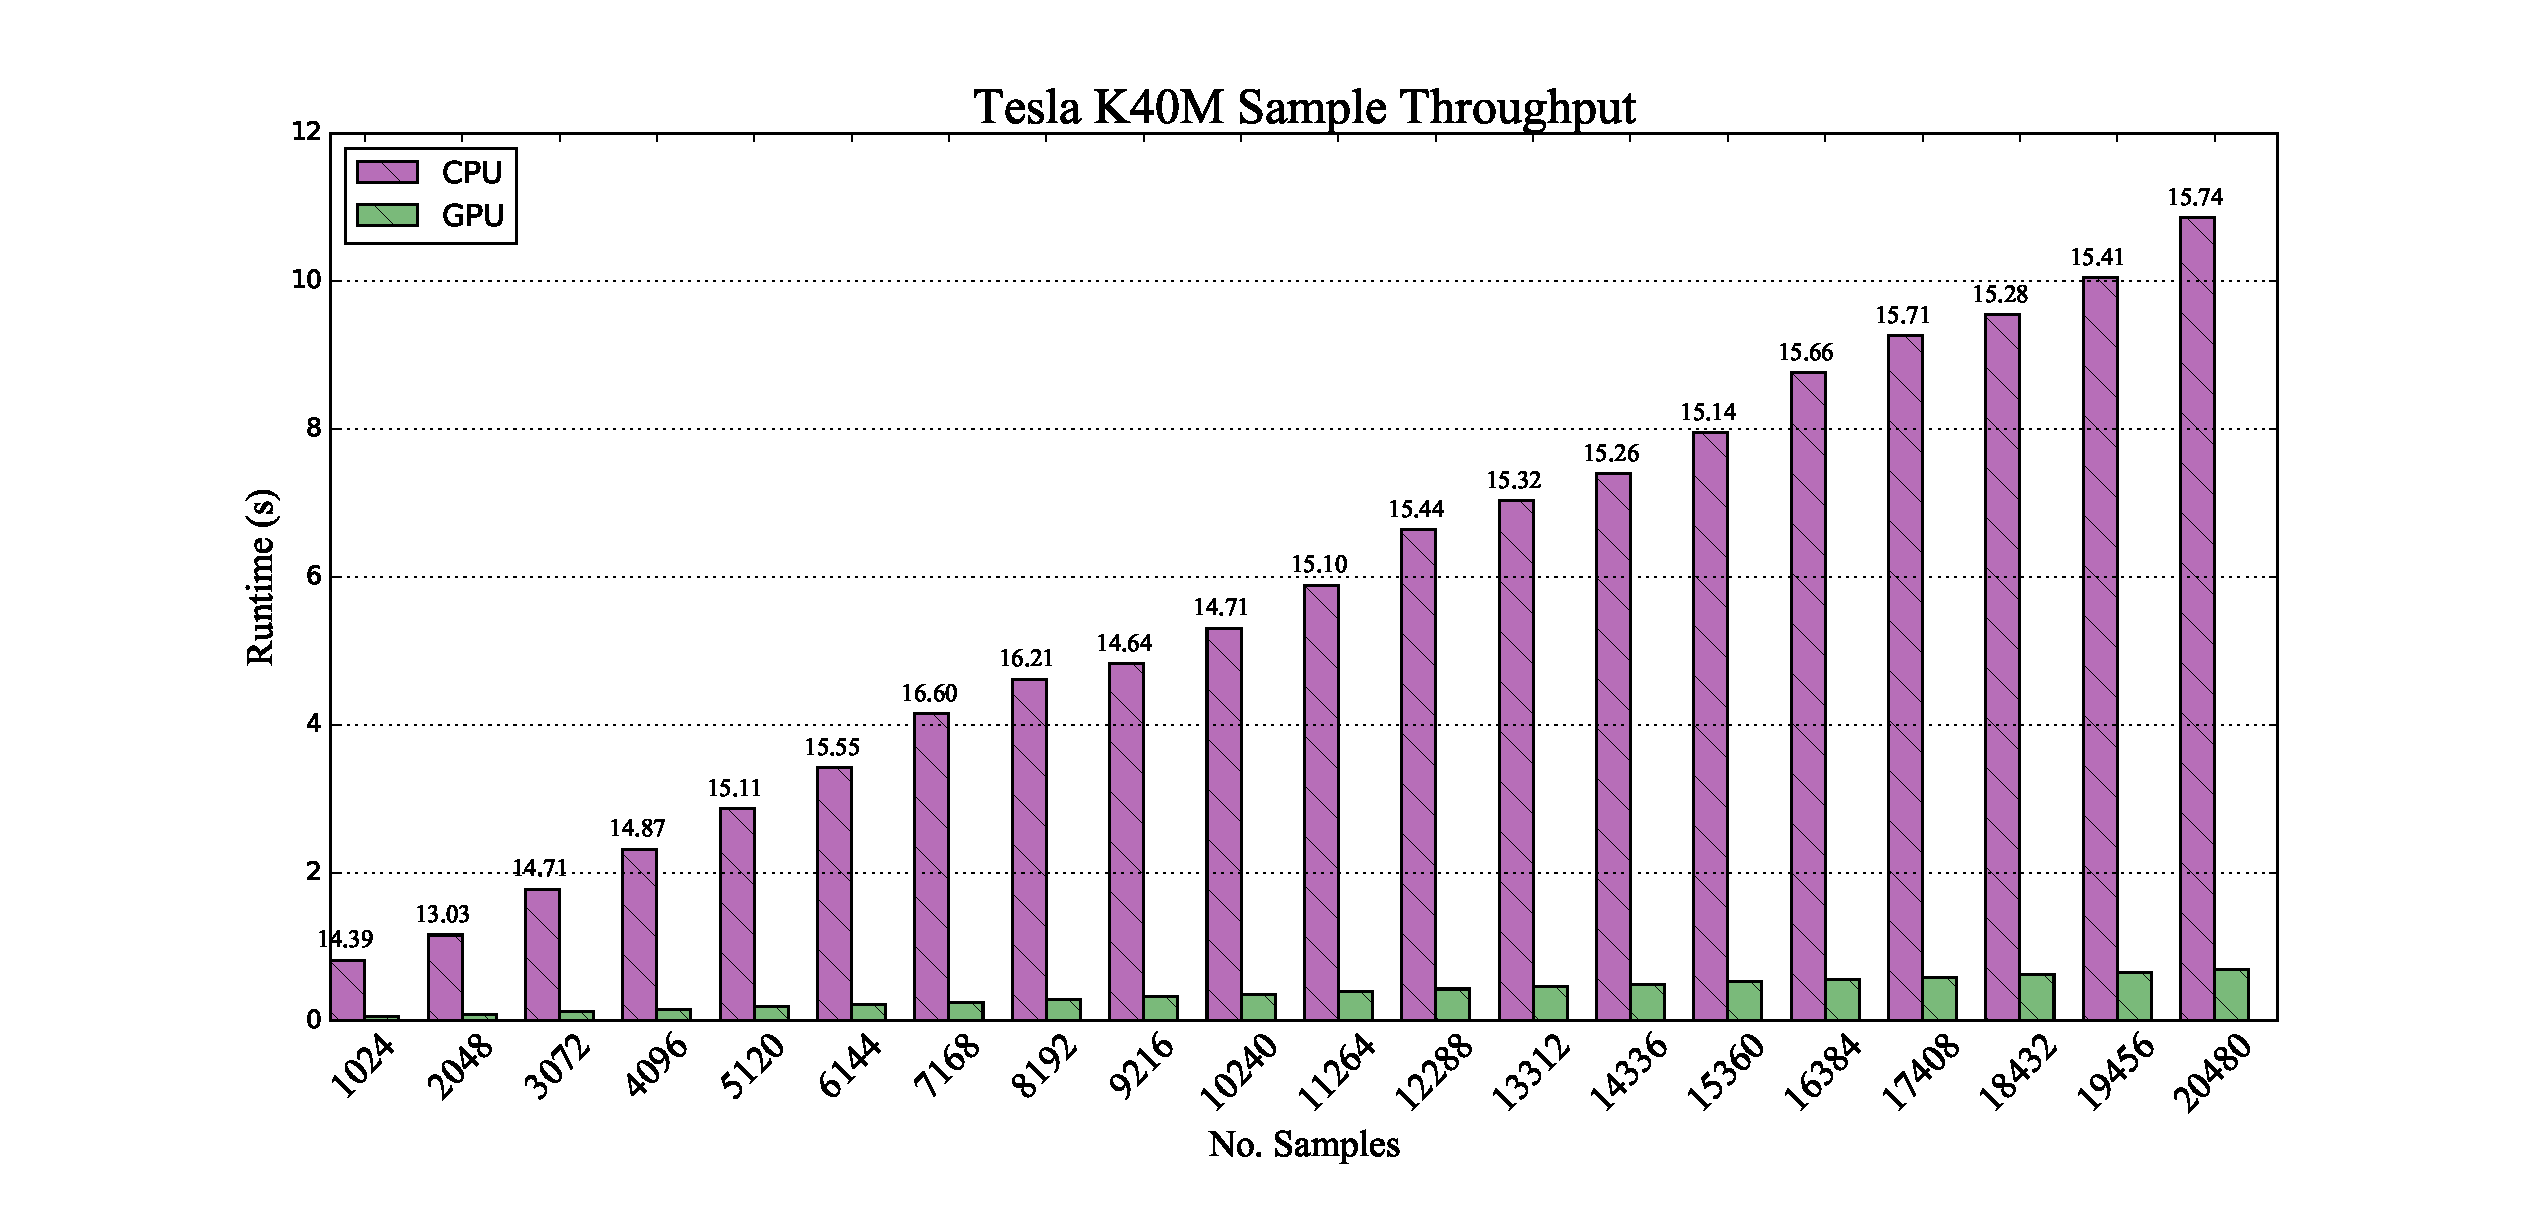
\includegraphics[scale=0.57]{speedup.eps}
\end{figure}

The dawn of gravitational wave astronomy in the 2015-2016 era has touched off a revolution in our ability to observe and classify astronomical phenomena. As with any entirely novel method of gleaning information from distant sources, development of methods to process and decipher such data has been explosive. Pure gravitational wave astrophysics has exciting prospects for the future, but the possibility of advancing other classical forms of astrophysics through their interplay with these newer methods is equally compelling. Significant research \cite{first2years} in th epast several years has been designed specifically to connect electromagnetic astronomy to gravitational wave observations, in particular the study of low-latency electromagnetic follow-up to gravitatioanl wave triggers. A central point of focus in these studies is the opportunity to give electromagnetic observers early warning on possible short duration transient events such as gamma ray bursts or longer duration klonovae. Such early warning could provide valuable insights as to the central engine of such gamma ray bursts and confirm recent models of these processes. However, electromagnetic observational resources are limited and expensive to operate and such it is imperative that any communication to such resources in the context of EM followup of GW triggers must be rapid and accurate to avoid wasting time and money. To that end it is desireable to develop existing parameter estimation codes to such a point that they can produces fast and correct results to reliably indicate potential sources of interest while minimizing false positives. The main goal of this work is to push this envelope and reduce the end-to-end runtime of parallel PE codes (specifically RapidPE) for the express purpose of low latency electromagnetic follow-up.

\subsection{Gamma Ray Bursts}
Gamma ray bursts (GRBs) are short duration transient events thought to occur during or shortly after the merger of compact binary systems, specifically those which include a single black hole and one neutron star. The presence of strong radiative emission from the poles of black holes has been confirmed by \cite{polarjet}, and while not yet directly observed, the interaction between such polar jets of radiation and the resulting post-merger NS remnant is a primary candidate for the generation of GRBs. The process is depicted in figure \textbf{FIGURE} in which an infalling NS is torn apart by the BH counterpart, leaving a remnant disk of energetic matter in orbit around the black hole. The radiation eminated from the poles of the BH impacts this disk and generates gamma rays, this is known as an internal shock. As the resulting cloud of matter ploughs into the surrounding interstellar medium, it slows, leaving a lower density region in its wake. Subsequent waves of matter may propagate through this region at a higher velocity then the initial blast wave, catching up and ramming into the back of the initial wave, producing further shocks.
It is not yet explicitly confirmed that this is the exact process by which GRBs are generated. It is generally accepted that to confirm this hypothesis we would need to observe direct coincidence between a GW trigger localized to some region of the sky and a GRB from the same direction. These phenomena have been demonstrated in numerical simulations by \cite{kilonova} and are highly dependent on initial system parameters. In particular the currently unknown commplete NS equation of state is known to play a pivotal role in braketing the mass and mass ratio ranges associated with GRB progenitors IIIIIII We now attempt to demonstrate the efficacy of the GPU based version of RapidPE for estimating these parammeters quickly and accurately. The frequency evolution of a compact binary system is given by the well known relationship

\begin{align}
\dot{f_{gw}}(\tau) = \frac{96}{5}\pi^{\frac{8}{3}} \left(\frac{G \mathcal{M}}{c^3}\right)^{\frac{5}{3}}f_{gw}^{\frac{11}{3}}
\end{align}

Integrating this equation we can find the total time during which a signal from such a binary remains in the Advanced LIGO frequency band:

\begin{align}\label{eq:timeinband}
\tau \approx 2.18s\left(\frac{1.21M_\odot}{\mathcal{M}}\right)^{\frac{5}{3}}\right)\left(\frac{100Hz}{f_{gw}}\right)^{\frac{8}{3}}
\end{align}

For calculational purposes the value $10Hz$ is used as $f_{gw}$ in the above equation, as this is the lower bound of reasonable sensitivity for ground based interferometers such as Advanced LIGO \textbf{CITATION}.

Numerical simulations have shown that NSBH fates are strongly sensitive to the initial binary mass ratio and equation of state. It has been found that systems for which approximately $q \gtrsim 4$ do not exhibit tidal disruption, the NS is swallowed whole by the BH before the tidal forces can overcome the NS self gravity. Since the largest NS masses are predicted \textbf{CITATION} to be approximately $1.4M_\odot$, the BH can be no larger then $\approx 5.6M_\odot$. This is equivalent to $\mathcal{M} \approx 2.33M_\odot$. Plugging this value into equation \ref{eq:timeinband} we find that such a system will spend approximately $5m 40s$ in the Advanced LIGO frequency band. 

\begin{figure}[H!]
\hspace{-0.5cm}
\includegraphics[scale=0.35]{gamray.png}
\end{figure}

\subsection{Kilonovae}
Compact binary mergers of neutron stars are thought to produce transient electromagnetic counterparts known as \textit{Kilonovae}. These smaller class of novae are dimmer and lower energy then regular novae or supernovae, and are hypothesized to occur due to the radiative emission of remnant matter displaced by the merger dynamics. It has been shown that a substantial fraction of elements heavier then Iron-56 are formed through r-process nucleosynthesis in the hearts of large stars, during which nuclei are subjected to high neutron flux as well as high electron density filling quantum states up to the Fermi energy. When this occurs $\beta^-$ decay of neutrons into protons is blocked \textit{CITATION} resulting in accumulation of large amounts of neutrons within the nuclei themselves. These nuclei later decay into heavy elements. These conditions are present during the merger of neutron stars or the tidal disruption of a neutron star by a black hole. Models of kilonovae have been successful in reproducing faint EM transients using r-process emission as a primary mechanism for radiation. Coincident measurements of such transients with localized gravitational waves is expected to be a smoking gun for confirming this model of kilonova genesis, thus it is important to assess the capability of modern parameter estimation to process signals from candidate systems and produce meaningful information useful for kilonova followup. 
Since merger ejecta from NSBH mergers is not subject to relativistic beaming, kilonovae emission is expected to be relatively isotropic. Assuming a random and uniform distribution of black hole spin directions there is thus an increased probability of detecting kilonovae of \textbf{SOLID ANGLE OVER 4 PI} relative to axially emissive GRBs. This translates to a better chance of finding a kilonova as a merger signature. Moreover, direct observation of kilonovae combined with numerical simulations can provide degeneracy-breaking information about the original progenitor through careful measurements of redshift compared to simulated spectra.   
The timescales characteristic of kilonova signatures are derived from numerical simulations, and most suggest a peak in the emission intensity roughly a day after merger. That said, the same simulations predict a steep rise in luminosity in the period just before the peak. For this reason crucial information about the astrophysics of kilonovae may be rapidly lost, and it is important to collect it as rapidly as possible. Figure \textbf{SOME FIGURE} depicts the timescales associated with kilonovae from \textbf{CITATION} as well as current PE methods prospects of convergence prior to certain features of the kilonova light curve.

\begin{figure}[H!]
\hspace{-6cm}
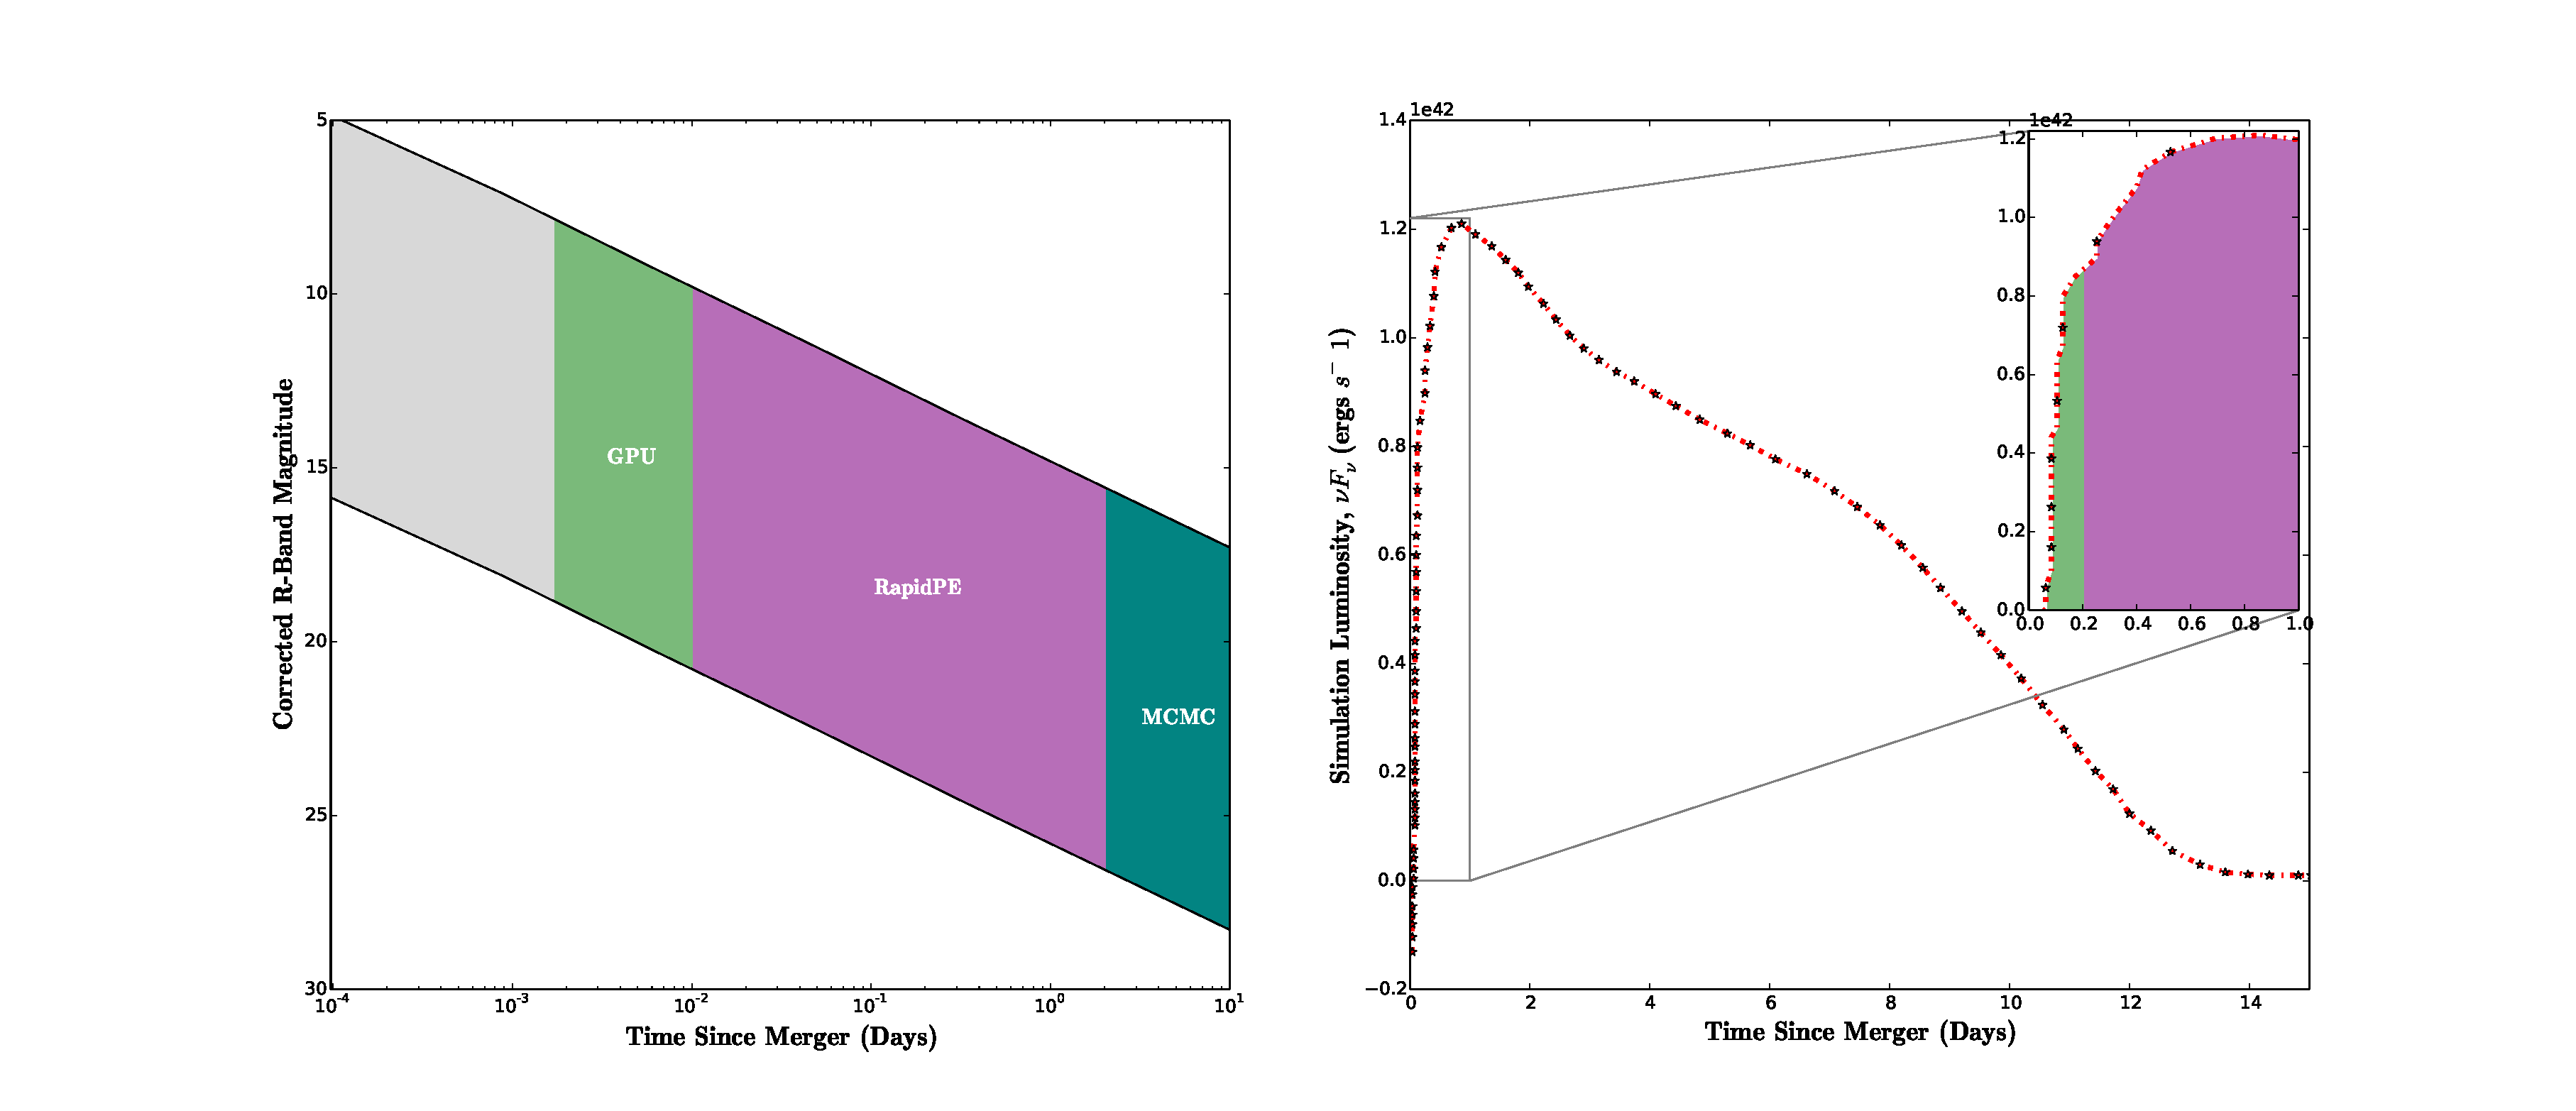
\includegraphics[scale=0.5]{EMFollow.eps}
\end{figure}


